% 线性方程Ax=b（上）：问题、解的情况、唯一解的求解方法（分解、例子、比较与核验）、无穷多解（解集与最小范数解）

\section{线性方程}
\label{sec:ls-exact-linear-equations}
\label{sec:linear-algebra-exact-systems}

给定矩阵$\bm A\in\mathbb R^{m\times d}$与目标$\bm b\in\mathbb R^m$，线性方程要求找出输入$\bm x$，
使$\bm A$作用后的输出恰好等于目标：
\begin{equation}
 \bm A\bm x=\bm b,\qquad \bm x\in\mathbb R^d.
 \label{eq:linear-algebra-linear-system}
\end{equation}
它由$m$个方程组成，含$d$个未知量。

若有$s$个目标$\bm b_1,\ldots,\bm b_s$共用同一个矩阵，
可以把它们排成$\bm B\in\mathbb R^{m\times s}$，把未知量排成$\bm X\in\mathbb R^{d\times s}$，
写成$\bm A\bm X=\bm B$。按矩阵乘法逐列读，这就是$s$个方程$\bm A\bm x_j=\bm b_j$并列。
每一列各自有解或无解，互不影响；它们只共享系数矩阵，因而可以共享对$\bm A$所做的计算。

本节按解的情况组织：先用秩判别方程有唯一解、有无穷多解还是没有解，再依次处理这三种情况，
并用伪逆把三种答案统一写出。这些讨论都假定数据精确；最后一部分借助第~\ref{chap:linear-analysis}章的条件数，
分析数据或计算有误差时解会偏离多少，并介绍降低误差影响的几种做法。

\subsection{解的情况}
\label{sec:ls-solution-cases}

按形状，$m=d$的方程称为方阵方程，$m>d$（方程多于未知量）称为超定，$m<d$（方程少于未知量）称为欠定。
一个自然的猜测是：超定方程无解，欠定方程多解，方阵方程恰有一解。下面的两个小方程说明这个猜测不成立。

\begin{example}[反例：形状不决定解的情况]
\label{ex:ls-shape-not-decisive}
超定方程
\[
 \begin{bmatrix}1\\1\end{bmatrix}x=\begin{bmatrix}1\\1\end{bmatrix}
\]
由两个相同的方程$x=1$组成，$x=1$是它的唯一解。方阵方程
\[
 \begin{bmatrix}1&1\\1&1\end{bmatrix}\bm x=\begin{bmatrix}1\\2\end{bmatrix}
\]
由$x_1+x_2=1$与$x_1+x_2=2$组成，两式左边相同而右边不同，互相矛盾，所以无解。
因此超定方程可以有唯一解，方阵方程也可以无解。
\end{example}

形状只限制了秩的上限：秩不超过$\min\{m,d\}$。有没有解要看$\bm b$与$\bm A$的列空间的关系，
有几个解要看$\bm A$的零空间，下面两段分别讨论。这里的“有解”指等式严格成立。
浮点计算中只能比较残差与容限，这一问题留到第~\ref{sec:ls-numerical-sensitivity}节；
算法报告失败，可能只是数值或实现上的问题，不能据此断定方程无解。

\paragraph{有解的条件}
\label{sec:ls-compatibility}

记$\bm a_1,\ldots,\bm a_d$为$\bm A$的各列。按矩阵乘法，$\bm A\bm x=x_1\bm a_1+\cdots+x_d\bm a_d$，
输入只提供组合系数。$\bm x$取遍$\mathbb R^d$时，输出恰好取遍列空间$\operatorname{range}(\bm A)$，所以
\[
 \bm A\bm x=\bm b\ \text{有解}\iff\bm b\in\operatorname{range}(\bm A).
\]
满足这一条件时称方程\term{相容}（consistent）。

为了能具体检验，把$\bm b$并到$\bm A$右侧，得到增广矩阵$[\bm A\;\bm b]$。
若$\bm b$已是原有列的组合，添上它不扩大列张成的空间，秩不变；否则新列带来一个新方向，秩恰好加一。因此
\begin{equation}
 \bm A\bm x=\bm b\ \text{相容}\iff
 \operatorname{rank}[\bm A\;\bm b]=\operatorname{rank}(\bm A).
 \label{eq:ls-augmented-rank}
\end{equation}
用示例~\ref{ex:ls-shape-not-decisive}中的方阵检验这一判据。

\begin{example}[增广矩阵的秩]
\label{ex:ls-augmented-rank-check}
取$\bm A=\left[\begin{smallmatrix}1&1\\1&1\end{smallmatrix}\right]$，它的两列相同，秩为$1$。右端取$\bm b=(1,2)^\top$时，
\[
 [\bm A\;\bm b]=\begin{bmatrix}1&1&1\\1&1&2\end{bmatrix}
\]
含线性无关的两列$(1,1)^\top$与$(1,2)^\top$，秩为$2>1$，所以方程无解，与示例~\ref{ex:ls-shape-not-decisive}的直接观察一致。
右端取$\bm b=(1,1)^\top$时，新列与原有的列相同，$[\bm A\;\bm b]$的秩仍为$1$，所以方程相容。
\end{example}

多右端方程$\bm A\bm X=\bm B$相容，当且仅当每一列$\bm b_j$都在列空间中，
即$\operatorname{rank}[\bm A\;\bm B]=\operatorname{rank}(\bm A)$。这些秩都可以用第~\ref{sec:ls-direct-methods}节的消元法求出。

\paragraph{解的个数}
\label{sec:ls-uniqueness-freedom}

方程相容以后，再问解有几个。若$\bm x_1,\bm x_2$都是解，则$\bm A(\bm x_1-\bm x_2)=\bm0$，两解之差落在零空间
$\operatorname{null}(\bm A)=\{\bm x:\bm A\bm x=\bm0\}$中；反过来，若$\bm x_0$是解且$\bm n\in\operatorname{null}(\bm A)$，
则$\bm A(\bm x_0+\bm n)=\bm b$，$\bm x_0+\bm n$也是解。所以方程相容时，任取一个解$\bm x_0$（称为特解），全部解恰为
\begin{equation}
 \bm x_0+\operatorname{null}(\bm A)=\{\bm x_0+\bm n:\bm n\in\operatorname{null}(\bm A)\}.
 \label{eq:ls-affine-solution-set}
\end{equation}
零空间只含零向量时解唯一；含有非零向量$\bm n$时，$\bm x_0+t\bm n$（$t\in\mathbb R$）已是无穷多个不同的解。
记$r=\operatorname{rank}(\bm A)$，由秩零度定理~\ref{thm:ls-rank-nullity}，$\dim\operatorname{null}(\bm A)=d-r$，
因此相容方程的解唯一，当且仅当$r=d$，即$\bm A$的$d$列线性无关，称为满列秩。

另一种满秩是$r=m$，称为满行秩。此时列空间是整个$\mathbb R^m$，任何右端都相容。
满行秩保证有解，满列秩保证有解时解唯一，下面的例子说明两种保证不能互换。

\begin{example}[反例：满行秩与满列秩互不蕴含]
\label{ex:ls-row-column-rank}
$1\times2$矩阵$\bm A=(1,1)$满行秩：方程$x_1+x_2=b$对每个$b$都有解；但$\bm A(1,-1)^\top=0$，
解可以沿$(1,-1)^\top$任意平移，不唯一。$2\times1$矩阵$\bm A=(1,1)^\top$满列秩：零空间只含零，有解必唯一；
但输出$x(1,1)^\top$的两个分量总相等，只有$\bm b\in\operatorname{span}\{(1,1)^\top\}$时才有解。
\end{example}

据此，超定方程即使满列秩，也只保证“有解则唯一”。欠定方程有$r\leq m<d$，有解时自由参数有$d-r\geq d-m\geq1$个，
所以从不唯一。方阵方程满秩时两种保证同时成立，对每个右端恰有一解，这正是$\bm A$可逆的情形。

\paragraph{方阵的行列式判据}
\phantomsection
\label{sec:ls-determinant-invertibility}
方阵是否可逆还可以由一个数判断。对$n$阶方阵$\bm A$，
\[
 \bm A\text{可逆}\iff\det\bm A\neq0,\qquad
 \bm A^{-1}=\frac{1}{\det\bm A}\operatorname{adj}(\bm A),\qquad
 \det(\bm A^{-1})=\frac{1}{\det\bm A}.
\]

若$\bm A$可逆，由行列式的乘法性（第~\ref{sec:ls-determinant-properties}节），$\det\bm A\det(\bm A^{-1})=\det\bm I_n=1$，
所以$\det\bm A\neq0$，并得第三式。反过来，若$\det\bm A\neq0$，把古典伴随恒等式
$\bm A\operatorname{adj}(\bm A)=\operatorname{adj}(\bm A)\bm A=(\det\bm A)\bm I_n$（定理~\ref{thm:ls-adjugate-identity}）两边除以$\det\bm A$，
就得到一个从左、右两侧乘$\bm A$都给出$\bm I_n$的矩阵，即第二式。二阶时，第二式就是第~\ref{sec:prelim-inverse-matrices}节的二阶求逆公式。

\begin{example}[用伴随矩阵求二阶逆]
\label{ex:ls-adjugate-two-by-two}
取$\bm A=\left[\begin{smallmatrix}2&1\\0&3\end{smallmatrix}\right]$。$\det\bm A=2\cdot3-1\cdot0=6\neq0$，所以$\bm A$可逆。
二阶矩阵的古典伴随由交换两个对角元、两个非对角元变号得到，于是
\[
 \bm A^{-1}=\frac16\begin{bmatrix}3&-1\\0&2\end{bmatrix}.
\]
乘回可验$\bm A\bm A^{-1}=\frac16\left[\begin{smallmatrix}6&0\\0&6\end{smallmatrix}\right]=\bm I_2$，
并且$\det(\bm A^{-1})=\frac1{36}(3\cdot2-0)=\frac16=1/\det\bm A$。
\end{example}

$\det\bm A=0$的几何含义是：单位立方体被$\bm A$压扁成体积为零的形状，列空间不是整个$\mathbb R^n$，有的右端无解。
所以$n$阶方阵方程对每个右端恰有一解，当且仅当$\operatorname{rank}\bm A=n$，也当且仅当$\det\bm A\neq0$。
行列式适合作理论判据，实际判断与求解时并不展开行列式：排列展开有$n!$项，
而第~\ref{sec:ls-direct-methods}节的消元在求解的同时就读出了秩。

\paragraph{三种情况的秩判别}

把两方面合起来，记$\tilde r=\operatorname{rank}[\bm A\;\bm b]$。由于添上一列至多使秩加一，总有$\tilde r=r$或$\tilde r=r+1$，
方程恰属于下面三种情况之一：
\[
 \begin{aligned}
  \tilde r&=r+1: &&\text{无解};\\
  \tilde r&=r=d: &&\text{唯一解};\\
  \tilde r&=r<d: &&\text{无穷多解，全部解含}\ d-r\ \text{个自由参数}.
 \end{aligned}
\]
示例~\ref{ex:ls-augmented-rank-check}的方阵中$r=1<d=2$：
右端$(1,2)^\top$使$\tilde r=2$，属于无解；右端$(1,1)^\top$使$\tilde r=1$，属于无穷多解。
下面三个小节依次处理唯一解、无穷多解与无解。

\subsection{唯一解的求解方法}
\label{sec:ls-direct-methods}
\label{sec:linear-algebra-direct-exact}
\label{sec:matrix-analysis-stable-solvers}

本小节讨论最常见的唯一解情形：$\bm A$是可逆方阵，对每个右端恰有一解。
超定而满列秩的方程在相容时也有唯一解，但判断它是否相容本身就要比较$\bm b$与列空间，
这与最小二乘的计算是同一件事，放到第~\ref{sec:ls-qr-method}节一并处理。

知道解唯一存在，还要把它算出来。三角方程最容易解：上三角方程的最后一个方程只含最后一个未知量，
解出后代入倒数第二个方程，又只剩一个未知量，如此从后向前逐个求出。

本小节的方法都把一般方程化成三角方程，或化成规模更小的方程，在有限步内得到精确算术下的精确解，称为直接法。
它们需要整体读取矩阵并存储分解因子，适合矩阵规模可控、或同一矩阵要配多个右端的情形。

不同方法利用不同的矩阵结构。我们从一般方阵的消元出发，得到LU分解；对称正定矩阵可以省去一半运算，
得到Cholesky分解；对称但不定的矩阵用LDL$^{\top}$分解；具有分块结构或只作低秩修改的矩阵，
可以把大方程化成小方程。用正交变换化三角的QR分解同样能解方程，它与最小二乘一起在第~\ref{sec:ls-qr-method}节讨论。
最后把这些方法的适用条件和代价并列比较，并说明算出的解怎样核验。

\subsubsection{消元与LU分解}

高斯消元用一个方程的倍数去消另一个方程中的未知量。三种行变换——把某行的倍数加到另一行、交换两行、
某行乘非零常数——都可以逆转，因而不改变解集。先看一个二阶的例子。

\begin{example}[二阶方程的消元]
\label{ex:ls-elimination-two-by-two}
解
\[
 \begin{bmatrix}2&1\\4&3\end{bmatrix}\bm x=\begin{bmatrix}1\\3\end{bmatrix},
\]
即$2x_1+x_2=1$、$4x_1+3x_2=3$。第二个方程减去第一个方程的$2$倍，消去$x_1$，得$x_2=1$。
代回第一个方程，$2x_1+1=1$，得$x_1=0$。所以唯一解是$\bm x=(0,1)^\top$。
\end{example}

\paragraph{消元乘子与LU因子}

阶数较高时，消元按列进行，每一步把一列主对角线以下的元素全部消成零。下面的例子显示，
记下每一步所用的倍数，就得到矩阵的一个乘积分解。

\begin{example}[三阶消元与LU分解]
\label{ex:ls-lu-three-by-three}
考虑方程
\[
 \bm A\bm x=\begin{bmatrix}2&1&1\\4&3&3\\8&7&9\end{bmatrix}\bm x
 =\begin{bmatrix}3\\7\\19\end{bmatrix},
\]
先只对系数矩阵$\bm A$消元。第一步以$a_{1,1}=2$为主元，即用来做除数的元素。
第二行减去第一行的$l_{2,1}=4/2=2$倍，变为$(0,1,1)$；第三行减去第一行的$l_{3,1}=8/2=4$倍，变为$(0,3,5)$。
第二步以新的$(2,2)$元$1$为主元，第三行减去第二行的$l_{3,2}=3/1=3$倍，变为$(0,0,2)$。
消元结束时剩下上三角矩阵$\bm U$，三个乘子按位置填进单位下三角矩阵$\bm L$：
\[
 \bm L=\begin{bmatrix}1&0&0\\2&1&0\\4&3&1\end{bmatrix},\qquad
 \bm U=\begin{bmatrix}2&1&1\\0&1&1\\0&0&2\end{bmatrix}.
\]
乘回可验$\bm L\bm U=\bm A$，例如$\bm L\bm U$的第三行是$4\cdot(2,1,1)+3\cdot(0,1,1)+(0,0,2)=(8,7,9)$。
\end{example}

图~\ref{fig:ls-lu-elimination-steps}画出这两步消元，以及乘子怎样按位置收集成$\bm L$。
乘回之所以能复原$\bm A$，是因为消元过程可以倒过来读。$\bm U$的第$i$行，是$\bm A$的第$i$行减去
若干个已经处理好的行（即$\bm U$的前$i-1$行）的倍数得到的，倍数就是乘子$l_{i,k}$：
\[
 \bm U_{i,:}=\bm A_{i,:}-\sum_{k<i}l_{i,k}\bm U_{k,:}
 \quad\Longrightarrow\quad
 \bm A_{i,:}=\sum_{k<i}l_{i,k}\bm U_{k,:}+1\cdot\bm U_{i,:}.
\]
右式说明$\bm A$的第$i$行是$\bm U$各行以$(l_{i,1},\ldots,l_{i,i-1},1,0,\ldots,0)$为系数的组合，
这正是$\bm L\bm U$的第$i$行。因此只要消元中不出现零主元，就有$\bm A=\bm L\bm U$，
其中$\bm L$是对角元为$1$的下三角矩阵，$\bm U$是上三角矩阵，称为LU分解。

有了分解，$\bm A\bm x=\bm b$就是$\bm L(\bm U\bm x)=\bm b$。令$\bm z=\bm U\bm x$，先从前向后解下三角方程
$\bm L\bm z=\bm b$（前代），再从后向前解上三角方程$\bm U\bm x=\bm z$（回代）：
\begin{equation}
 z_i=b_i-\sum_{j<i}l_{i,j}z_j,\qquad
 x_i=\frac{z_i-\sum_{j>i}u_{i,j}x_j}{u_{i,i}}.
\end{equation}
下面用这两个公式完成示例~\ref{ex:ls-lu-three-by-three}的求解。

\begin{example}[用LU因子前代与回代]
\label{ex:ls-lu-forward-back}
沿用示例~\ref{ex:ls-lu-three-by-three}的因子$\bm L,\bm U$与右端$\bm b=(3,7,19)^\top$。前代解$\bm L\bm z=\bm b$：
\[
 z_1=3,\qquad z_2=7-2\cdot3=1,\qquad z_3=19-4\cdot3-3\cdot1=4.
\]
回代解$\bm U\bm x=\bm z$：
\[
 x_3=\frac42=2,\qquad x_2=\frac{1-1\cdot x_3}{1}=-1,
\]
\[
 x_1=\frac{3-1\cdot x_2-1\cdot x_3}{2}=1.
\]
代回原方程，$\bm A(1,-1,2)^\top=(3,7,19)^\top$，所以$\bm x=(1,-1,2)^\top$是方程的解。
\end{example}

前代算出的$\bm z$，正是消元过程对右端做同样变换的结果：例如$z_2=7-2\cdot3$，
就是第二行减去第一行的$2$倍时右端的变化。
\begin{figure}[!htb]
  \centering
  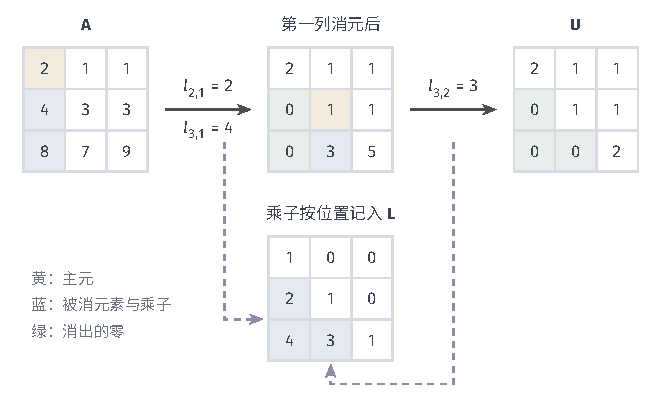
\includegraphics[width=112mm]{figures/00-shared/mathematical-preliminaries-upper/02-linear-spaces/tikz/comprehension-additions/linear-lu-elimination-steps.pdf}
  \caption{三阶矩阵的消元与LU因子。左起依次是$\bm A$、消去第一列后的矩阵与$\bm U$；
  黄色是当前主元，蓝色是待消去的元素，绿色是消出的零。箭头上的乘子等于被消元素除以主元，
  下方按原位置收集成单位下三角因子$\bm L$，满足$\bm L\bm U=\bm A$。}
  \label{fig:ls-lu-elimination-steps}
\end{figure}

\paragraph{选主元}

上面的做法要求每一步的主元不为零。可逆矩阵也可能在主元位置出现零，例如
$\left[\begin{smallmatrix}0&1\\1&1\end{smallmatrix}\right]$的$(1,1)$元为零，无法用它做除数；
交换两行后，以$1$为主元即可继续。主元不为零但很小时，问题同样存在，只是在浮点计算中才暴露出来。
下面的例子用只保留三位有效数字的算术显示这一点。

\begin{example}[小主元与行交换]
\label{ex:ls-partial-pivoting}
解$\left[\begin{smallmatrix}10^{-4}&1\\1&1\end{smallmatrix}\right]\bm x=(1,2)^\top$，
精确解为$x_1=1/(1-10^{-4})\approx1.0001$、$x_2=2-x_1\approx0.9999$。设每步运算结果
只保留三位有效数字（教学设定）。

不交换时，以$10^{-4}$为主元，乘子$l_{2,1}=10^4$。消元后右下角系数
$1-10^4=-9999$舍入为$-1.00\times10^4$，右端$2-10^4=-9998$也舍入为
$-1.00\times10^4$，得$x_2=1.00$，回代$x_1=(1-1.00)/10^{-4}=0$，第一分量完全错误：
大乘子把第二行原有的“$1$”和“$2$”淹没在$10^4$量级中。

先交换两行，以$1$为主元，乘子$l_{2,1}=10^{-4}$。消元后右下角系数$1-10^{-4}$与右端$1-2\times10^{-4}$
都舍入为$1.00$，得$x_2=1.00$，回代$x_1=2-1.00=1.00$，两分量在三位精度下都正确。
两种做法在精确算术中给出同一个解，区别只在乘子大小。
\end{example}

示例~\ref{ex:ls-partial-pivoting}说明，主元比同列其他元素小得多时，乘子会很大，舍入误差随之被放大。
因此第$k$步先在第$k$列尚未处理的元素中选绝对值最大的一个，把它所在的行换到主元位置，再消元。
这种做法称为部分主元，它保证每个乘子满足$|l_{i,k}|\leq1$。把全部行交换累计成置换矩阵$\bm P$，
得到带部分主元的LU分解
\begin{equation}
 \bm P\bm A=\bm L\bm U,
 \label{eq:matrix-analysis-palu}
\end{equation}
求解时先把右端按同样的方式重排，依次解$\bm L\bm z=\bm P\bm b$与$\bm U\bm x=\bm z$。
行交换只改变方程的排列次序，不改变解集。若示例~\ref{ex:ls-lu-three-by-three}也用部分主元，
第一步会把含$8$的第三行换到顶部，得到另一组$\bm P,\bm L,\bm U$，解不变。

行交换不会把奇异矩阵变成可逆矩阵。若某一步在精确算术下，当前列尚未处理的元素全为零，找不到非零主元，
说明这一列是前面主元列的组合，矩阵秩亏。这时跳过该列，继续处理下一列，最后得到阶梯形，非零主元的个数就是秩。

这样，消元同时回答了第~\ref{sec:ls-solution-cases}节的问题。
在阶梯形中，若某行左边全为零而右端非零，即出现$0=c\neq0$的矛盾行，方程不相容，这与增广矩阵的秩判据一致；
若没有矛盾行，把不对应主元的未知量（自由变量）取零，回代即得一个特解，其余解沿零空间展开，
具体做法见第~\ref{sec:ls-select-among-solutions}节。

浮点计算中，一个很小的主元并不能证明矩阵精确奇异：代数上的奇异（主元恰为零）与数值上的接近奇异
（主元很小但非零）是两回事，后者用数值秩描述，见第~\ref{sec:ls-numerical-sensitivity}节。

\paragraph{代价、复用与填充}

稠密$d\times d$矩阵的LU分解约需$2d^3/3$次浮点运算，$\bm L$与$\bm U$可以覆盖原矩阵存放，存储为$O(d^2)$。
分解完成后，每个右端只需前代与回代各一次，运算量为$O(d^2)$。所以同一个$\bm A$配多个右端$\bm b_j$时，
分解只做一次，此后每列只付$O(d^2)$的代价。复用的前提是矩阵不变；矩阵元素一旦改变，旧的$\bm L\bm U$
不再等于新的$\bm P\bm A$，必须重新分解，或改用后文的低秩更新。

稀疏矩阵的情形更微妙。消元会在原来为零的位置产生非零元，称为\term{填充}（fill-in），
使原本稀疏的因子变得接近稠密。填充的多少取决于消元顺序，下面的箭头形矩阵说明这一点。

\begin{example}[箭头形矩阵的填充]
\label{ex:ls-arrow-fill-in}
考虑一个$5\times5$矩阵，其中一个变量与其余全部变量耦合，其余变量彼此不耦合，
非零元只在对角线和这个变量对应的行与列上。

若先消去这个变量，要从其余每一行减去它所在行的倍数，而这一行在所有列上都有非零元，
所以剩下的$4\times4$块全部变成非零：原来只有$4$个对角非零元，现在有$16$个，新增的$12$个都是填充。
若把它排到最后，消去前四个变量时，每一步只改动右下角那一个元素，不产生任何填充。

推广到$n$阶，前一种顺序使因子变为稠密，需存约$n^2$个元素，分解约需$O(n^3)$次运算；
后一种只需原有的$3n-2$个元素和$O(n)$次运算。
\end{example}

图~\ref{fig:ls-sparse-fill-in-ordering}并置了两种顺序。矩阵和解都相同，代价却随顺序相差悬殊，
所以稀疏直接法先选消元顺序、再作分解，其代价也不能只按原始非零元数估计。
\begin{figure}[!htb]
  \centering
  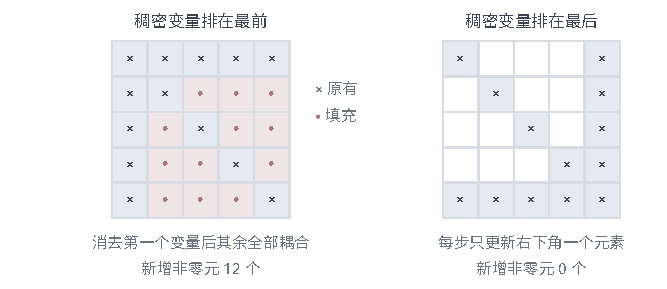
\includegraphics[width=112mm]{figures/00-shared/mathematical-preliminaries-upper/02-linear-spaces/tikz/comprehension-additions/linear-sparse-fill-in-ordering.pdf}
  \caption{消元顺序决定填充。同一个“箭头形”矩阵：左图把与全部变量耦合的变量排在最前，
  消去它后其余位置全部变为非零（红点为填充）；右图把它排在最后，因子保持原有稀疏结构。
  蓝格是原矩阵的非零元。}
  \label{fig:ls-sparse-fill-in-ordering}
\end{figure}

\subsubsection{Cholesky分解}

很多方程的系数矩阵是对称正定的，例如第~\ref{sec:ls-least-squares}节满列秩时的$\bm A^\top\bm A$。
对这类矩阵，LU分解有两处浪费：$\bm U$与$\bm L$实际上携带同样的信息（$\bm U$的第$i$行是$\bm L^\top$的第$i$行乘以第$i$个主元），却要分别计算和存储；
部分主元的行交换会破坏对称性，而对称正定矩阵其实不需要交换。下面说明，对称正定矩阵可以写成
$\bm L\bm L^\top$，只算一个三角因子，并且不必选主元。

设$\bm A=\bm A^\top\succ0$。把第一行、第一列与其余部分分开，也把待求的下三角因子同样分块：
\[
 \bm A=\begin{bmatrix}a_{1,1}&\bm a^\top\\\bm a&\bm A_{22}\end{bmatrix},\qquad
 \bm L=\begin{bmatrix}l_{1,1}&\bm0\\\bm l&\bm L_{22}\end{bmatrix},\qquad
 \bm L\bm L^\top=\begin{bmatrix}l_{1,1}^2&l_{1,1}\bm l^\top\\ l_{1,1}\bm l&\bm l\bm l^\top+\bm L_{22}\bm L_{22}^\top\end{bmatrix}.
\]
令$\bm L\bm L^\top=\bm A$并逐块比较：左上角要求$l_{1,1}^2=a_{1,1}$。正定性给出
$a_{1,1}=\bm e_1^\top\bm A\bm e_1>0$，故可取$l_{1,1}=\sqrt{a_{1,1}}>0$。左下角要求$\bm l=\bm a/l_{1,1}$。
右下角要求
\[
 \bm L_{22}\bm L_{22}^\top=\bm A_{22}-\bm l\bm l^\top=\bm A_{22}-\frac{\bm a\bm a^\top}{a_{1,1}},
\]
问题化为对低一阶的矩阵$\bm A_{22}-\bm a\bm a^\top/a_{1,1}$做同样的分解。

这个剩余矩阵仍然对称正定。对任意非零$\bm u$，取$\bm x=(-\bm a^\top\bm u/a_{1,1},\,\bm u)$，它非零，展开可得
$\bm x^\top\bm A\bm x=\bm u^\top(\bm A_{22}-\bm a\bm a^\top/a_{1,1})\bm u$，而左边为正。
右边正是对第一个变量配方后剩下的二次型。于是同样的论证可以一阶一阶做下去，每一步开方的数都严格为正。
定理~\ref{thm:ls-gram-factor}用同样的配方归纳证明了正定矩阵可写成$\bm L^\top\bm L$的形式，
那里的上三角因子就是这里的$\bm L^\top$；这里把同一构造落实为逐列计算的算法。

\paragraph{Cholesky因子的逐列构造}

总结起来，对称正定矩阵$\bm A$存在唯一的对角元为正的下三角矩阵$\bm L$，使
\begin{equation}
 \bm A=\bm L\bm L^\top,
 \label{eq:matrix-analysis-cholesky}
\end{equation}
称为\term{Cholesky分解}（Cholesky decomposition）。上面的分块递推展开成逐元素的形式，就是按列计算
\begin{equation}
 l_{j,j}=\sqrt{a_{j,j}-\sum_{k<j}l_{j,k}^2},\qquad
 l_{i,j}=\frac{a_{i,j}-\sum_{k<j}l_{i,k}l_{j,k}}{l_{j,j}}\quad(i>j).
\end{equation}
两式都来自比较$\bm L\bm L^\top$与$\bm A$的元素：$\bm L\bm L^\top$的$(i,j)$元（$i\geq j$）是
$\sum_{k\leq j}l_{i,k}l_{j,k}$，其中$k<j$的项只含前面各列，已经算出；剩下的一项$l_{i,j}l_{j,j}$
（$i=j$时是$l_{j,j}^2$）便可解出。根号内的数是第$j$步配方后的剩余，正定性保证它严格为正。
唯一性也由此可见：每个元素都被唯一解出，只有开方有正负两种选择，约定对角元为正就排除了这一任意性。
下面按这两个公式算一个三阶的例子。

\begin{example}[逐列计算Cholesky因子]
\label{ex:ls-cholesky-three-by-three}
取对称矩阵
$\bm A=\left[\begin{smallmatrix}4&2&2\\2&5&3\\2&3&6\end{smallmatrix}\right]$。
第一列：$l_{1,1}=\sqrt4=2$，$l_{2,1}=2/2=1$，$l_{3,1}=2/2=1$。此时剩余矩阵为
\[
 \begin{bmatrix}5&3\\3&6\end{bmatrix}-\begin{bmatrix}1&1\\1&1\end{bmatrix}
 =\begin{bmatrix}4&2\\2&5\end{bmatrix}.
\]
第二列：$l_{2,2}=\sqrt{5-l_{2,1}^2}=\sqrt4=2$，$l_{3,2}=(3-l_{3,1}l_{2,1})/l_{2,2}=(3-1)/2=1$。
第三列：$l_{3,3}=\sqrt{6-l_{3,1}^2-l_{3,2}^2}=\sqrt4=2$。于是
\[
 \bm L=\begin{bmatrix}2&0&0\\1&2&0\\1&1&2\end{bmatrix},
\]
乘回$\bm L\bm L^\top$逐项等于$\bm A$。三个根号内的数都是$4$，都为正。
\end{example}

计算本身也是正定性的检验。若每一步根号内的数都为正，就得到可逆的$\bm L$，
于是对非零$\bm x$有$\bm x^\top\bm A\bm x=\lVert\bm L^\top\bm x\rVert_2^2>0$，$\bm A$正定；
反之，若某一步根号内出现零或负数，$\bm A$就不是正定的。示例~\ref{ex:ls-cholesky-three-by-three}的计算因此同时证明了$\bm A$正定。

求解时，依次解$\bm L\bm z=\bm b$（前代，$z_i=(b_i-\sum_{j<i}l_{i,j}z_j)/l_{i,i}$）与
$\bm L^\top\bm x=\bm z$（回代，$x_i=(z_i-\sum_{j>i}l_{j,i}x_j)/l_{i,i}$）。

\begin{example}[用Cholesky因子求解]
\label{ex:ls-cholesky-solve}
沿用示例~\ref{ex:ls-cholesky-three-by-three}的$\bm A$与$\bm L$，取右端$\bm b=(8,10,11)^\top$。前代解$\bm L\bm z=\bm b$：
\[
 z_1=\frac82=4,\qquad z_2=\frac{10-1\cdot4}{2}=3,\qquad z_3=\frac{11-1\cdot4-1\cdot3}{2}=2.
\]
回代解$\bm L^\top\bm x=\bm z$：
\[
 x_3=\frac22=1,\qquad x_2=\frac{3-1\cdot1}{2}=1,\qquad x_1=\frac{4-1\cdot1-1\cdot1}{2}=1.
\]
代回可验$\bm A(1,1,1)^\top=(8,10,11)^\top$，所以$\bm x=(1,1,1)^\top$。
\end{example}

稠密情形的运算量约为$d^3/3$，是LU的一半；存储也只需一个三角因子，约$d^2/2$个元素。多个右端同样复用一次分解。

矩阵只是半正定时，某一步的配方剩余可能恰为零，后续除以$l_{j,j}$就无法进行。
这时不应随手给对角线加一个小常数让计算通过，那样解的已经是另一个方程。
应先分清原因：$\bm A$本身有零空间时，方程不再有唯一解，回到第~\ref{sec:ls-solution-cases}节判断它属于哪种情况；
剩余量只是因舍入而接近零时，属于数值问题，见第~\ref{sec:ls-numerical-sensitivity}节。
只有任务本身要求加入惩罚项时，才改解相应的正则化方程（第~\ref{sec:ls-regularized-ls}节）。

\subsubsection{LDL$^{\top}$分解}
\label{sec:ls-ldlt}

对称但不定的矩阵，既有使二次型为正的方向，也有使它为负的方向。前面已经说明，逐列计算成功就证明矩阵正定，
所以对不定矩阵，Cholesky的开方必定在某一步遇到非正的数。下面是最小的例子。

\begin{example}[反例：不定矩阵的Cholesky中断]
\label{ex:ls-cholesky-indefinite}
取$\bm A=\left[\begin{smallmatrix}1&2\\2&1\end{smallmatrix}\right]$。它对称，$\det\bm A=-3\neq0$，所以可逆；
但$\bm x=(1,-1)^\top$给出$\bm x^\top\bm A\bm x=1-4+1=-2<0$，$\bm A$不定。按Cholesky的逐列公式，
第一列得$l_{1,1}=1$、$l_{2,1}=2$，第二列要求
\[
 l_{2,2}=\sqrt{a_{2,2}-l_{2,1}^2}=\sqrt{1-2^2}=\sqrt{-3},
\]
在实数中无法进行。
\end{example}

我们仍想利用对称性，只算一个三角因子。办法是不开方，把每一步的主元单独放进对角矩阵$\bm D$，负号就留在$\bm D$里。

\paragraph{LDL$^{\top}$因子的形成}

仍以示例~\ref{ex:ls-cholesky-indefinite}的矩阵为例，看不开方时消元记录下什么。

\begin{example}[二阶不定矩阵的LDL$^{\top}$分解]
\label{ex:ls-ldlt-two-by-two}
对$\bm A=\left[\begin{smallmatrix}1&2\\2&1\end{smallmatrix}\right]$，以$a_{1,1}=1$为主元，乘子$l_{2,1}=2/1=2$，
消元后剩余系数为$1-2\cdot2=-3$。把乘子放进单位下三角矩阵，把两个主元$1$与$-3$放进对角矩阵，得
\[
 \bm A=\begin{bmatrix}1&0\\2&1\end{bmatrix}
 \begin{bmatrix}1&0\\0&-3\end{bmatrix}
 \begin{bmatrix}1&2\\0&1\end{bmatrix}=\bm L\bm D\bm L^\top .
\]
乘回可验等式成立。剩余系数$-3$原样保留在$\bm D$中，不需要开方。
\end{example}

这就是LDL$^{\top}$分解的基本形式：$\bm L$是单位下三角矩阵，$\bm D$是对角矩阵。

只用一阶主元并不总够，下面的矩阵就没有可用的一阶主元。

\begin{example}[反例：没有一阶主元的对称可逆矩阵]
\label{ex:ls-no-scalar-pivot}
取$\bm A=\left[\begin{smallmatrix}0&1\\1&0\end{smallmatrix}\right]$。$\det\bm A=-1\neq0$，所以$\bm A$可逆；
但两个对角元都是零，没有一个能作除数。若像LU那样交换两行，得到的是$\bm P\bm A=\bm L\bm U$形式的分解，
不再是对称的$\bm L\bm D\bm L^\top$。若对称地交换，即同时交换两行和对应的两列，结果仍是$\bm A$本身：
对称置换只重新排列对角元，而这里的对角元全为零。
\end{example}

所以解决办法有两条。一是对称地交换，矩阵仍然对称，对角元被重新排列；若其他位置有合适的对角元，
就可以把它换到主元位置。二是允许用$2\times2$的对称可逆块作主元，在对角元都不合适时必须这样做：
示例~\ref{ex:ls-no-scalar-pivot}的整个矩阵就是一个可逆的二阶块，直接把它放进$\bm D$即可。
一般地，把对称置换累计成$\bm P$，得到
\[
 \bm P\bm A\bm P^\top=\bm L\bm D\bm L^\top,
\]
其中$\bm L$单位下三角，$\bm D$由一阶与二阶对角块组成。

计算过程与LU相同，只是按块进行。把当前待处理的矩阵分块为
$\left[\begin{smallmatrix}\bm A_{11}&\bm A_{21}^\top\\\bm A_{21}&\bm A_{22}\end{smallmatrix}\right]$，
其中$\bm A_{11}$是选定的可逆一阶或二阶主元块。正如标量消元用乘子$l_{i,k}=a_{i,k}/a_{k,k}$，
块消元的乘子块是$\bm L_{21}=\bm A_{21}\bm A_{11}^{-1}$；从下面的块行中减去$\bm L_{21}$乘主元块行，
左下块变成零，右下块变成
\[
 \bm A_{22}-\bm L_{21}\bm A_{21}^\top=\bm A_{22}-\bm A_{21}\bm A_{11}^{-1}\bm A_{21}^\top ,
\]
它仍是对称矩阵，对它重复同样的过程。$\bm L$收集各步的乘子块，$\bm D$收集各步的主元块。
每一步都可以把$\bm L\bm D\bm L^\top$乘回，核对它是否等于置换后的矩阵。

求解时先把右端按$\bm P$重排，再依次解下三角方程$\bm L\bm z=\bm P\bm b$、
块对角方程$\bm D\bm y=\bm z$与上三角方程$\bm L^\top\bm w=\bm y$，最后令$\bm x=\bm P^\top\bm w$还原次序。
其中块对角方程逐块求解：一阶块$d$直接得$y=z/d$；二阶块
$\left[\begin{smallmatrix}d_{11}&d_{12}\\d_{12}&d_{22}\end{smallmatrix}\right]$
的行列式$\Delta=d_{11}d_{22}-d_{12}^2$因主元块可逆而非零，由二阶逆矩阵公式得
\begin{equation}
 y_1=\frac{d_{22}z_1-d_{12}z_2}{\Delta},\qquad
 y_2=\frac{d_{11}z_2-d_{12}z_1}{\Delta}.
\end{equation}
示例~\ref{ex:ls-no-scalar-pivot}的二阶块有$\Delta=-1$，代入得$y_1=z_2$、$y_2=z_1$，
两个未知量一次解出。与Cholesky相比，这一求解过程只是在两次三角求解之间插入了块对角求解，并多了置换与还原；
运算量同样约为$d^3/3$。

最后要分清$\bm D$中的两种情况。负的对角元或不定的二阶块表示矩阵有负方向，但它们可逆，
方程照样唯一可解；零块则表示矩阵奇异，不能当作可逆块做除法，需要回到第~\ref{sec:ls-solution-cases}节重新判断解的情况。

\subsubsection{分块消元与低秩更新}
\label{sec:matrix-analysis-blocks-updates}

LDL$^{\top}$分解中的块消元有更广的用途。若未知量可以自然地分成两组，而且消去其中一组很便宜，
就可以先消去它，只解剩下那组未知量满足的较小方程。先看每组只有一个未知量的最小例子。

\begin{example}[二阶方程的分块消元]
\label{ex:ls-block-elimination-two-by-two}
解$\left[\begin{smallmatrix}2&1\\1&2\end{smallmatrix}\right](x_1,x_2)^\top=(1,3)^\top$。
第一个方程$2x_1+x_2=1$给出$x_1=(1-x_2)/2$。代入第二个方程$x_1+2x_2=3$，得
\[
 \frac{1-x_2}{2}+2x_2=3,\qquad\text{即}\qquad \frac32x_2=3-\frac12=\frac52,
\]
故$x_2=5/3$，回代得$x_1=(1-5/3)/2=-1/3$。核验：$2(-1/3)+5/3=1$，$(-1/3)+2(5/3)=3$。
消去$x_1$后，$x_2$的系数从$2$变成$2-1\cdot\tfrac12\cdot1=\tfrac32$，右端从$3$变成$3-1\cdot\tfrac12\cdot1=\tfrac52$。
\end{example}

图~\ref{fig:ls-schur-block-elimination}把这两步并置。下面把标量换成块，看系数与右端的这两处变化在一般情形下是什么。

\begin{figure*}[htbp]
  \centering
  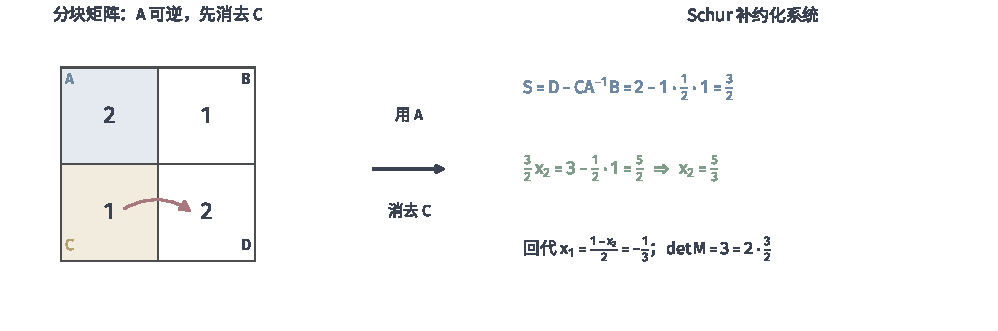
\includegraphics[width=168.998mm]{figures/00-shared/mathematical-preliminaries-upper/02-linear-spaces/matplotlib/ls-schur-block-elimination/ls-schur-block-elimination.pdf}
  \caption{Schur 补的 2×2 分块消元。左：$\bm M=\left[\begin{smallmatrix}2&1\\1&2\end{smallmatrix}\right]$
  按左上块$\bm A=2$分块，先由第一行表出$x_1=(1-x_2)/2$；右：代入第二行后右下角残留
  Schur补$\bm S=3/2$，约化得$x_2=5/3$、回代$x_1=-1/3$，且$\det\bm M=2\cdot3/2=3$。
  解析式教学构造。}
  \label{fig:ls-schur-block-elimination}
\end{figure*}

\paragraph{Schur补与约化系统}

设分块方程为
\[
 \begin{bmatrix}\bm A&\bm B\\\bm C&\bm D\end{bmatrix}
 \begin{bmatrix}\bm x\\\bm y\end{bmatrix}
 =\begin{bmatrix}\bm f\\\bm g\end{bmatrix},
\]
系数矩阵记为$\bm M$，其中$\bm A\in\mathbb R^{p\times p}$可逆。第一组方程$\bm A\bm x+\bm B\bm y=\bm f$
给出$\bm x=\bm A^{-1}(\bm f-\bm B\bm y)$；代入第二组$\bm C\bm x+\bm D\bm y=\bm g$，得
$\bm C\bm A^{-1}\bm f-\bm C\bm A^{-1}\bm B\bm y+\bm D\bm y=\bm g$。整理后，$\bm y$满足
\begin{equation}
 \bm S\bm y=\bm g-\bm C\bm A^{-1}\bm f,
 \qquad
 \bm S=\bm D-\bm C\bm A^{-1}\bm B.
 \label{eq:matrix-analysis-schur-complement}
\end{equation}
矩阵$\bm S$称为$\bm A$在$\bm M$中的\term{Schur补}（Schur complement），方程~\eqref{eq:matrix-analysis-schur-complement}
称为约化系统。
\label{def:matrix-analysis-schur-complement}
示例~\ref{ex:ls-block-elimination-two-by-two}相当于取$\bm A=2$、$\bm B=\bm C=1$、$\bm D=2$、$\bm f=1$、$\bm g=3$，
此时$\bm S=2-1/2=3/2$，约化系统的右端为$3-1/2=5/2$，与那里算出的系数和右端一致。
Cholesky每一步的剩余矩阵$\bm A_{22}-\bm a\bm a^\top/a_{1,1}$，以及LDL$^{\top}$每一步的右下块，都是这样的Schur补。

同一过程写成矩阵乘法，是左乘一个单位块下三角矩阵，消去左下块：
\[
 \begin{bmatrix}\bm I&\bm0\\-\bm C\bm A^{-1}&\bm I\end{bmatrix}
 \begin{bmatrix}\bm A&\bm B\\\bm C&\bm D\end{bmatrix}
 =\begin{bmatrix}\bm A&\bm B\\\bm0&\bm S\end{bmatrix}.
\]
左边第一个因子的行列式为$1$，右边是块上三角矩阵，所以$\det\bm M=\det\bm A\det\bm S$。
因此在$\bm A$可逆的前提下，$\bm M$可逆当且仅当$\bm S$可逆。示例~\ref{ex:ls-block-elimination-two-by-two}中$\det\bm M=3=2\cdot\tfrac32$。

计算时，先解约化系统得到$\bm y$，再回代$\bm x=\bm A^{-1}(\bm f-\bm B\bm y)$。其中凡是出现$\bm A^{-1}$的地方，
都通过对$\bm A$的分解求解来实现，例如$\bm A^{-1}\bm B$由解$\bm A\bm Z=\bm B$得到，不必先形成逆矩阵。
这种做法的典型来源是二部结构：少量全局未知量与大量局部未知量相连，局部未知量彼此之间不直接耦合。
这时$\bm A$是块对角的，消去局部块很便宜，只剩下全局未知量的小系统。

若需要整个逆矩阵，把上述消元过程对一般右端做完，可得块逆公式
\begin{equation}
 \bm M^{-1}=
 \begin{bmatrix}
  \bm A^{-1}+\bm A^{-1}\bm B\bm S^{-1}\bm C\bm A^{-1}
  &-\bm A^{-1}\bm B\bm S^{-1}\\
  -\bm S^{-1}\bm C\bm A^{-1}&\bm S^{-1}
 \end{bmatrix}.
 \label{eq:matrix-analysis-block-inverse}
\end{equation}

$\bm M$对称时$\bm C=\bm B^\top$，Schur补还能判断正定性。对二次型配方：
\begin{equation}
 \begin{bmatrix}\bm x\\\bm y\end{bmatrix}^{\top}
 \bm M\begin{bmatrix}\bm x\\\bm y\end{bmatrix}
 =\bm x^\top\bm A\bm x+2\bm x^\top\bm B\bm y+\bm y^\top\bm D\bm y
 =(\bm x+\bm A^{-1}\bm B\bm y)^\top
 \bm A(\bm x+\bm A^{-1}\bm B\bm y)+\bm y^\top\bm S\bm y,
\end{equation}
展开右边第一项即可验证第二个等号，它多出的$\bm y^\top\bm B^\top\bm A^{-1}\bm B\bm y$正好被$\bm S=\bm D-\bm B^\top\bm A^{-1}\bm B$
中的减项抵消。于是在$\bm A\succ0$时
\begin{equation}
 \bm M\succ0\quad\Longleftrightarrow\quad
 \bm D-\bm B^\top\bm A^{-1}\bm B\succ0.
 \label{eq:matrix-analysis-schur-positive-definite}
\end{equation}
必要性：对任意非零$\bm y$，取$\bm x=-\bm A^{-1}\bm B\bm y$使第一项为零，二次型只剩$\bm y^\top\bm S\bm y$，它必须为正。
充分性：两项都非负；若和为零，则$\bm y^\top\bm S\bm y=0$迫使$\bm y=\bm0$，再由第一项为零得$\bm x=\bm0$。
Cholesky中剩余矩阵保持正定，正是这一结论的特例。

$\bm A$奇异时上述公式不能使用。此时第一组方程$\bm A\bm x=\bm f-\bm B\bm y$本身未必有解，
要求$\bm f-\bm B\bm y$落在$\operatorname{range}(\bm A)$中，至少需要$\operatorname{range}(\bm B)\subseteq\operatorname{range}(\bm A)$
之类的条件，而且$\bm A$的零空间还会给$\bm x$留下自由参数，须按第~\ref{sec:ls-solution-cases}节的判别另行处理。

\paragraph{Woodbury恒等式与小系统}

另一类常见情形是：$\bm A$已经分解好，矩阵却改成了$\bm A+\bm U\bm C\bm V^\top$，其中
$\bm U,\bm V\in\mathbb R^{d\times k}$，$\bm C\in\mathbb R^{k\times k}$，$k$远小于$d$。
例如在最小二乘中增加或删除一条观测，系数矩阵就改变一个秩一项。这里的修改是精确的，不是近似。
重新分解需要$O(d^3)$次运算；能否借旧分解，只解一个$k$阶的小方程？

可以，办法是引入辅助未知量，把问题改写成分块方程，再用上面的Schur补。设$\bm C$可逆，要解
$(\bm A+\bm U\bm C\bm V^\top)\bm x=\bm b$。令$\bm z=\bm C\bm V^\top\bm x\in\mathbb R^k$，原方程等价于
\[
 \bm A\bm x+\bm U\bm z=\bm b,\qquad \bm V^\top\bm x-\bm C^{-1}\bm z=\bm0 .
\]
按约化系统的做法消去$\bm x$：由第一式$\bm x=\bm A^{-1}(\bm b-\bm U\bm z)$，代入第二式得
$\bm V^\top\bm A^{-1}\bm b-\bm V^\top\bm A^{-1}\bm U\bm z-\bm C^{-1}\bm z=\bm0$，即
\[
 (\bm C^{-1}+\bm V^\top\bm A^{-1}\bm U)\bm z=\bm V^\top\bm A^{-1}\bm b .
\]
这是一个$k$阶方程。记它的系数矩阵为$\bm S=\bm C^{-1}+\bm V^\top\bm A^{-1}\bm U$，设其可逆，
则$\bm z=\bm S^{-1}\bm V^\top\bm A^{-1}\bm b$，代回得
$\bm x=\bm A^{-1}\bm b-\bm A^{-1}\bm U\bm S^{-1}\bm V^\top\bm A^{-1}\bm b$。
这对每个$\bm b$都成立，因此得到\term{Woodbury恒等式}
\begin{equation}
 (\bm A+\bm U\bm C\bm V^\top)^{-1}
 =\bm A^{-1}-\bm A^{-1}\bm U
 (\bm C^{-1}+\bm V^\top\bm A^{-1}\bm U)^{-1}
 \bm V^\top\bm A^{-1}.
 \label{eq:matrix-analysis-woodbury}
\end{equation}
使用时同样不形成逆矩阵：用旧分解解出$\bm A^{-1}\bm b$和$\bm A^{-1}\bm U$（共$k+1$个右端，每个右端一次前代、一次回代，代价$O(d^2)$），
形成并求解$k$阶小方程，再组合出$\bm x$，总代价为$O(kd^2+k^3)$。前提是$\bm A$可逆且已有分解，
小矩阵$\bm S$可逆；$\bm S$接近奇异时公式对误差敏感。最常用的是$\bm C=\bm I$，此时只要求
$\bm A$与$\bm I+\bm V^\top\bm A^{-1}\bm U$可逆，对矩形的$\bm U,\bm V$不需要任何逆。

$k=1$时$\bm U=\bm u$、$\bm V=\bm v$是向量，取$\bm C=1$，小方程变成标量方程，得到Sherman--Morrison公式
\[
 (\bm A+\bm u\bm v^\top)^{-1}
 =\bm A^{-1}-\frac{\bm A^{-1}\bm u\bm v^\top\bm A^{-1}}
 {1+\bm v^\top\bm A^{-1}\bm u},
 \qquad 1+\bm v^\top\bm A^{-1}\bm u\neq0 .
\]

行列式也有相应的公式。对上面的分块矩阵
$\left[\begin{smallmatrix}\bm A&\bm U\\\bm V^\top&-\bm C^{-1}\end{smallmatrix}\right]$，
先消左上块，行列式是$\det\bm A\det(-\bm S)$；改为先消右下块$-\bm C^{-1}$，对应的Schur补是
$\bm A-\bm U(-\bm C^{-1})^{-1}\bm V^\top=\bm A+\bm U\bm C\bm V^\top$，行列式是$\det(-\bm C^{-1})\det(\bm A+\bm U\bm C\bm V^\top)$。
两者相等，$k$阶矩阵前的负号各带出$(-1)^k$而抵消，得
$\det(\bm A+\bm U\bm C\bm V^\top)=\det\bm A\det\bm C\det\bm S$。

下面用一个二阶例子核对更新公式与行列式公式。

\begin{example}[秩一更新的求解]
\label{ex:ls-sherman-morrison-update}
取$\bm A=\operatorname{diag}(2,3)$、$\bm u=\bm v=(1,1)^\top$、$\bm b=(1,0)^\top$。
新矩阵是$\bm A+\bm u\bm v^\top=\left[\begin{smallmatrix}3&1\\1&4\end{smallmatrix}\right]$，直接求解得$\bm x=(4/11,-1/11)^\top$。
改用更新公式，只需对旧矩阵$\bm A$求解：
\[
 \bm A^{-1}\bm b=(1/2,\,0)^\top,\qquad
 \bm A^{-1}\bm u=(1/2,\,1/3)^\top,
\]
\[
 1+\bm v^\top\bm A^{-1}\bm u=1+\tfrac12+\tfrac13=\tfrac{11}6,\qquad
 \bm v^\top\bm A^{-1}\bm b=\tfrac12 .
\]
于是小方程的解为$z=(1/2)/(11/6)=3/11$，
\[
 \bm x=\bm A^{-1}\bm b-z\,\bm A^{-1}\bm u
 =\begin{bmatrix}1/2\\0\end{bmatrix}-\frac3{11}\begin{bmatrix}1/2\\1/3\end{bmatrix}
 =\begin{bmatrix}4/11\\-1/11\end{bmatrix},
\]
与直接求解一致。行列式公式给出$\det\bm A\cdot\tfrac{11}6=6\cdot\tfrac{11}6=11$，也与$3\cdot4-1\cdot1=11$一致。
\end{example}

\subsubsection{方法比较与选择}
\label{sec:ls-direct-method-comparison}

上面各方法做的是同一件事：用消元或正交变换把方程化为三角方程或更小的方程。区别在于
各自要求矩阵具备什么结构，以及利用这种结构省下多少运算、存储，稳定性如何。
表~\ref{tab:ls-direct-method-comparison}把这些差别并列，并把第~\ref{sec:ls-qr-method}节的QR一并列入以便比较。
运算量按稠密$d\times d$矩阵（QR按$m\times d$）计；稀疏矩阵的实际代价还取决于消元顺序产生的填充。

\begin{table*}[htbp]
 \centering\small
 \begin{tabularx}{\linewidth}{@{}l>{\raggedright\arraybackslash}X>{\raggedright\arraybackslash}p{24mm}>{\raggedright\arraybackslash}X>{\raggedright\arraybackslash}X>{\raggedright\arraybackslash}X@{}}
  \toprule
  方法 & 适用矩阵 & 稠密运算量 & 存储 & 稳定性 & 典型用途\\
  \midrule
  LU（部分主元） & 一般可逆方阵；秩亏时消元暴露秩与矛盾行 & $2d^3/3$ & $\bm L,\bm U$覆盖原矩阵，另存置换 & 乘子满足$\lvert l_{i,k}\rvert\leq1$，实践中稳定；最坏情形的元素增长极少出现 & 无对称结构的方阵方程；同一矩阵配多个右端\\
  Cholesky & 对称正定 & $d^3/3$ & 一个三角因子，约$d^2/2$个元素 & 不选主元即稳定；根号内出现非正数即说明矩阵不正定 & 满列秩的正规方程、协方差矩阵与核矩阵；也用来检验正定性\\
  LDL$^{\top}$ & 对称不定、可逆 & 约$d^3/3$ & 一个三角因子与块对角$\bm D$ & 需对称选主元（一阶或二阶块）控制乘子；$\bm D$的负块记录负方向 & 等式约束二次优化的最优性方程等鞍点系统\\
  QR & 任意$m\geq d$矩阵，满列秩时回代唯一 & $2md^2-2d^3/3$，方阵约$4d^3/3$ & 反射向量与$\bm R$，约$md$个元素 & 正交变换不放大误差，不形成$\bm A^\top\bm A$ & 超定最小二乘、近秩亏问题（第~\ref{sec:ls-qr-method}节）\\
  分块消元 & 被消去的块可逆，其余块耦合稀疏 & 由被消块的分解与Schur补的阶数决定 & 各块因子与Schur补 & 取决于被消块与Schur补的条件，被消块接近奇异时不可靠 & 二部结构，如三维重建中先消去大量三维点、只解相机参数块\\
  Woodbury & 已分解矩阵加秩$k$修改，$k\ll d$ & 已有因子时$O(kd^2+k^3)$ & 旧因子、修改因子与$k$阶小矩阵 & 小系统接近奇异时敏感 & 增删一条观测后更新解（$k=1$即Sherman--Morrison）\\
  \bottomrule
 \end{tabularx}
 \caption{线性方程直接解法的比较。从上到下，前三种按对称性与正定性逐步收窄适用范围、
 换取更低的运算与存储；QR以更高运算量换取不形成$\bm A^\top\bm A$；后两种不是独立分解，
 而是借已有求解器把大系统化为小系统。}
 \label{tab:ls-direct-method-comparison}
\end{table*}

选择方法时，按结构由特殊到一般逐项检查，越特殊的结构能省下越多代价。

第一，看是否已有分解、矩阵只作了低秩修改，或者矩阵有可以先消去的分块结构。
例如矩阵形如$\bm G=\sum_i\bm a_i\bm a_i^\top$时（第~\ref{sec:ls-least-squares}节的正规方程就是这种形式），
每新增一条观测$\bm a$，$\bm G$只增加一个秩一项$\bm a\bm a^\top$，用Sherman--Morrison借旧分解更新解只需$O(d^2)$，
重新分解则需$O(d^3)$。

第二，看对称性与正定性。上面的$\bm G$在各$\bm a_i$张成全空间时对称正定，用Cholesky最省。
对称而不定的矩阵则不能用Cholesky。

一个典型的对称不定矩阵来自带等式约束的二次优化。在正定二次目标上加等式约束，
其最优性条件（\BookChapterRef{chap:optimization}{第~\ref{chap:optimization}章}的KKT条件）是以
$\left[\begin{smallmatrix}\bm H&\bm C^\top\\\bm C&\bm0\end{smallmatrix}\right]$
为系数矩阵的线性方程，其中$\bm H\succ0$、$\bm C\neq\bm0$。这个矩阵对称，取$\bm y=\bm0$、$\bm x\neq\bm0$可得正方向，
但它也必有负方向：取$\bm y$使$\bm C^\top\bm y\neq\bm0$，再取$\bm x=-\bm H^{-1}\bm C^\top\bm y$，
代入前面的配方公式（其中$\bm A=\bm H$、$\bm B=\bm C^\top$、$\bm D=\bm0$），第一项为零，第二项是
$\bm y^\top(\bm0-\bm C\bm H^{-1}\bm C^\top)\bm y=-(\bm C^\top\bm y)^\top\bm H^{-1}(\bm C^\top\bm y)<0$。
所以它要用LDL$^{\top}$或LU。

第三，没有对称结构时，用部分主元LU。最后，若问题本身是超定的最小二乘，或列之间接近线性相关，
用QR比先形成正规方程更可靠。无论选哪一种，都要先核对前提：把不定矩阵交给Cholesky，
会在某一步遇到非正的配方剩余而中断；把奇异的被消块交给分块消元，约化系统根本无法形成。

\subsubsection{结果核验}
\label{sec:ls-linear-equation-verification}

算出$\bm x$后还要确认它确实满足原方程。三角方程或约化系统解对了，不等于原方程成立：
置换是否还原、乘子是否记错、小系统的解是否正确回代，都只能回到原方程检查。
具体做法是计算残差$\bm r=\bm b-\bm A\bm x$，报告$\lVert\bm r\rVert$或相对残差
$\lVert\bm r\rVert/\lVert\bm b\rVert$（$\bm b\neq\bm0$时），与任务给定的容限比较；多右端时逐列计算，
不能用一列的残差代替另一列。以示例~\ref{ex:ls-elimination-two-by-two}为例，解出$\bm x=(0,1)^\top$，
代回得$\bm A\bm x=(1,3)^\top$，残差为零。

所用方法的前提也要复核：Cholesky要求对称正定，LDL$^{\top}$要求所选主元块可逆，分块消元要求被消去的块可逆。
若计算中途发现矩阵奇异，结论就不再是“解唯一”，应按第~\ref{sec:ls-solution-cases}节给出可复核的依据：
无解时给出消元中出现的矛盾行，多解时给出一个特解和零空间的一组基。

最后，残差小只说明$\bm x$几乎满足方程，不说明$\bm x$离真解近。矩阵接近奇异时，
很小的残差可能对应很大的解误差。第~\ref{chap:linear-analysis}章的条件数正是误差与残差之间的放大倍数，
它对线性方程的具体含义见第~\ref{sec:ls-numerical-sensitivity}节。

\subsection{无穷多解}
\label{sec:ls-select-among-solutions}

秩亏而相容时，即$\operatorname{rank}[\bm A\;\bm b]=\operatorname{rank}(\bm A)=r<d$，方程有无穷多解。
这时要做两件事：先把全部解描述清楚，并算出描述所需的特解与零空间的基；
再说明若只报告一个答案，应当报告哪一个，以及怎样计算它。

\subsubsection{解集的结构}
\label{sec:linear-algebra-affine-relations}

第~\ref{sec:ls-uniqueness-freedom}节已经证明，全部解是$\bm x_0+\operatorname{null}(\bm A)$，
即把子空间$\operatorname{null}(\bm A)$平移到某个特解$\bm x_0$处得到的集合。这样的集合称为\term{仿射空间}（affine space）。
基点$\bm x_0$可以换成任何别的解，集合本身不变；方向空间$\operatorname{null}(\bm A)$则由集合唯一确定，
因为它恰好由集合中任意两点之差组成。例如$x_1+x_2=2$有特解$(1,1)^\top$，
零空间由$(1,-1)^\top$张成，全部解为$(1,1)^\top+t(1,-1)^\top$，$t\in\mathbb R$。

换个角度看，按“输出是否相同”把输入分组，同一组中任意两点之差都在零空间中，每组正是零空间的一个平移。
方程$\bm A\bm x=\bm b$的解集，就是输出为$\bm b$的那一组。
图~\ref{fig:vol1-add-linear-nullspace-fibers}以$\bm A=(1,1)$画出这种分组：
每条平行线$x_1+x_2=c$上的点产生同一个输出$c$。
\begin{figure}[!htb]
  \centering
  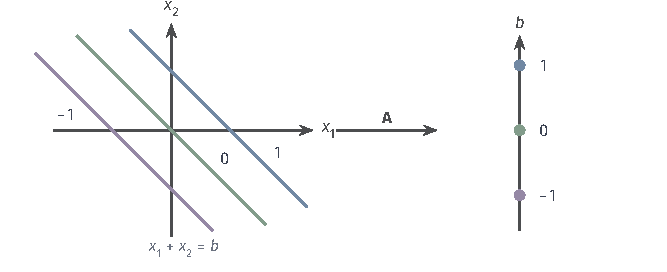
\includegraphics[width=112mm]{figures/00-shared/mathematical-preliminaries-upper/02-linear-spaces/tikz/comprehension-additions/linear-nullspace-fibers.pdf}
  \caption{同一输出对应的整组输入。对$\bm A=(1,1)$，蓝、绿、紫直线分别满足
  $x_1+x_2=1,0,-1$；右侧同色点是各直线的输出。绿色直线是$\ker\bm A$，
  其余直线是它的平移。把一整条直线归为一类后，才得到与可达输出的一一对应。}
  \label{fig:vol1-add-linear-nullspace-fibers}
\end{figure}

解集有多大，由零空间的维数决定。$\dim\operatorname{null}(\bm A)=d-r$，取零空间的一组基$\bm n_1,\ldots,\bm n_{d-r}$，
全部解可写成$\bm x_0+t_1\bm n_1+\cdots+t_{d-r}\bm n_{d-r}$，其中$t_1,\ldots,t_{d-r}$任意取值，
所以解集有$d-r$个自由参数。上例中$d=2$、$r=1$，自由参数只有$t$一个。

\paragraph{特解与零空间基的计算}

这一描述需要两样东西：一个特解和零空间的一组基。二者都可以从消元得到的阶梯形读出
（第~\ref{sec:ls-direct-methods}节）。主元所在的列对应主元变量，其余未知量称为自由变量，共$d-r$个。
把全部自由变量取零，回代解出主元变量，就得到一个特解；把右端换成零，令某一个自由变量取$1$、其余取零，
回代得到零空间中的一个向量，依次对每个自由变量这样做，得到的$d-r$个向量线性无关，构成零空间的一组基。
下面的例子按这一步骤计算。

\begin{example}[从阶梯形读出特解与零空间的基]
\label{ex:ls-particular-null-basis}
解
\[
 \begin{bmatrix}1&2&1\\2&4&3\end{bmatrix}\bm x=\begin{bmatrix}4\\9\end{bmatrix}.
\]
第二行减去第一行的$2$倍，得阶梯形
\[
 \begin{bmatrix}1&2&1\\0&0&1\end{bmatrix}\bm x=\begin{bmatrix}4\\1\end{bmatrix},
\]
即$x_3=1$。主元在第一、三列，$x_2$是自由变量，$r=2$、$d-r=1$。取$x_2=0$，
回代$x_1=4-2x_2-x_3=3$，得特解$\bm x_0=(3,0,1)^\top$。右端换成零并取$x_2=1$，得$x_3=0$、$x_1=-2$，
零空间由$\bm n=(-2,1,0)^\top$张成。所以全部解为
\[
 \bm x=(3-2t,\,t,\,1)^\top,\qquad t\in\mathbb R .
\]
代回可验$\bm A\bm x_0=(4,9)^\top$、$\bm A\bm n=\bm0$。
\end{example}

\subsubsection{最小范数解}

方程本身给出的是整个仿射空间$\bm x_0+\operatorname{null}(\bm A)$，并不指定其中哪一个点。
若要报告一个确定的答案，必须另加准则。
最常用的准则是取欧氏范数最小的解，几何上就是在仿射空间中找离原点最近的点。

准则需要事先声明，因为不同准则选出的点不同：换一个内积，离原点“最近”的点一般也会改变。
示例~\ref{ex:ls-particular-null-basis}的特解$(3,0,1)^\top$也是一个合法的解，
只是它来自“自由变量取零”这一约定，换一种消元顺序就会得到另一个特解。

为求范数最小的点，把输入分成两部分：被$\bm A$消去的部分和真正决定输出的部分。
第一部分属于$\operatorname{null}(\bm A)$；第二部分应取在它的正交补中。
由定理~\ref{thm:ls-four-subspaces-orthogonality}，这个正交补就是行空间，$\operatorname{null}(\bm A)^\perp=\operatorname{range}(\bm A^\top)$，
输入空间有正交直和$\mathbb R^d=\operatorname{range}(\bm A^\top)\oplus\operatorname{null}(\bm A)$（式~\eqref{eq:ls-four-subspaces-decomposition}）：
$\operatorname{null}(\bm A)$是被消去的输入方向，$\operatorname{range}(\bm A^\top)$是真正影响输出的方向。

\paragraph{最小范数精确解的唯一性}

按输入空间的分解，每个解唯一写成$\bm x=\bm x_R+\bm x_N$，其中$\bm x_R\in\operatorname{range}(\bm A^\top)$，
$\bm x_N\in\operatorname{null}(\bm A)$。所有解共有同一个$\bm x_R$：若$\bm x'=\bm x'_R+\bm x'_N$是另一个解，
则$\bm x_R-\bm x'_R=(\bm x-\bm x')-(\bm x_N-\bm x'_N)$既在$\operatorname{range}(\bm A^\top)$中，
又是两个零空间向量之差，落在$\operatorname{null}(\bm A)$中；两个子空间互相正交，只交于零向量，故$\bm x_R=\bm x'_R$。
由于$\bm A\bm x_N=\bm0$，$\bm A\bm x_R=\bm A\bm x=\bm b$，$\bm x_R$本身也是解。两部分正交，勾股恒等式给出
\[
 \lVert\bm x\rVert_2^2=\lVert\bm x_R\rVert_2^2+\lVert\bm x_N\rVert_2^2\geq\lVert\bm x_R\rVert_2^2,
\]
等号当且仅当$\bm x_N=\bm0$。所以最小范数解存在且唯一，就是解集中落在$\operatorname{range}(\bm A^\top)$里的那一个。
用前面的直线方程核对这一刻画。

\begin{example}[直线$x_1+x_2=2$上的最小范数解]
\label{ex:ls-min-norm-line}
方程$x_1+x_2=2$的系数矩阵为$\bm A=(1,1)$，全部解为$(1+t,1-t)^\top$，$t\in\mathbb R$。它们的范数平方为
\[
 (1+t)^2+(1-t)^2=2+2t^2,
\]
在$t=0$时最小，所以最小范数解是$(1,1)^\top$。它正比于$\bm A^\top=(1,1)^\top$，确实落在$\operatorname{range}(\bm A^\top)$中。
\end{example}

\paragraph{最小范数解的计算}

这一刻画也给出计算方法。设$\bm A$满行秩，要找的解形如$\bm x=\bm A^\top\bm w$，代入方程得
$\bm A\bm A^\top\bm w=\bm b$。$m$阶方阵$\bm A\bm A^\top$可逆：若$\bm A\bm A^\top\bm w=\bm0$，
则$\lVert\bm A^\top\bm w\rVert_2^2=\bm w^\top\bm A\bm A^\top\bm w=0$，即$\bm A^\top\bm w=\bm0$，
而$\bm A^\top$的$m$列线性无关，迫使$\bm w=\bm0$。于是最小范数解为
\[
 \bm x=\bm A^\top(\bm A\bm A^\top)^{-1}\bm b .
\]
实际计算时不形成逆矩阵：$\bm A\bm A^\top$对称正定，先用Cholesky分解解出$\bm w$，再算$\bm A^\top\bm w$。

\begin{example}[满行秩方程的最小范数解]
\label{ex:ls-min-norm-row-full-rank}
示例~\ref{ex:ls-particular-null-basis}的系数矩阵$\bm A=\left[\begin{smallmatrix}1&2&1\\2&4&3\end{smallmatrix}\right]$的秩为$2$，满行秩。计算
\[
 \bm A\bm A^\top=\begin{bmatrix}6&13\\13&29\end{bmatrix},
\]
解$\bm A\bm A^\top\bm w=(4,9)^\top$得$\bm w=(-1/5,2/5)^\top$，于是
\[
 \bm x=\bm A^\top\bm w=(3/5,\,6/5,\,1)^\top .
\]
它是全部解$(3-2t,t,1)^\top$中$t=6/5$的那一个，与零空间方向$(-2,1,0)^\top$正交。
它的范数平方为$14/5$，小于特解$(3,0,1)^\top$的范数平方$10$。
\end{example}

矩阵$\bm A^\top(\bm A\bm A^\top)^{-1}$从右边乘$\bm A$得到单位矩阵，是第~\ref{sec:prelim-inverse-matrices}节介绍过的右逆中的一个。
右逆不唯一，其他右逆给出的一般不是最小范数解。

\begin{example}[反例：其他右逆不给出最小范数解]
\label{ex:ls-other-right-inverse}
取$\bm A=(1,1)$。右逆$\bm A^\top(\bm A\bm A^\top)^{-1}=(1/2,1/2)^\top$把$b$送到最小范数解$(b/2,b/2)^\top$，范数为$|b|/\sqrt2$。
$(1,0)^\top$也满足$\bm A(1,0)^\top=1$，是另一个右逆；它把$b$送到$(b,0)^\top$。这也是方程的解，
但范数为$|b|$，$b\neq0$时大于最小范数。
\end{example}

形成$\bm A\bm A^\top$会把各行之间接近线性相关的程度放大（第~\ref{sec:ls-normal-equations-method}节对$\bm A^\top\bm A$说明了同样的现象）。
更可靠的做法是对$\bm A^\top$作第~\ref{chap:linear-representation}章的经济型QR分解~\eqref{eq:ls-qr-factorization}，
$\bm A^\top=\bm Q\bm R$，$\bm Q$是$d\times m$矩阵，$\bm R$是$m$阶可逆上三角矩阵。
最小范数解落在$\operatorname{range}(\bm A^\top)=\operatorname{range}(\bm Q)$中，可写成$\bm x=\bm Q\bm w$。
代入方程，$\bm A\bm x=\bm R^\top\bm Q^\top\bm Q\bm w=\bm R^\top\bm w=\bm b$，
这是下三角方程，前代即得$\bm w$。所得的解与上面的公式相同，但不形成$\bm A\bm A^\top$；
QR分解怎样稳定地计算，见第~\ref{sec:ls-orthogonalization-qr}节。

$\bm A$不满行秩时，有些方程可以由其他方程组合出来，$\bm A\bm A^\top$不可逆，上面的公式不能直接使用。
方程相容时，可以先删去这些多余的方程，化为满行秩的情形；要把最小范数解写成一个矩阵作用于$\bm b$，
则需要第~\ref{sec:ls-pseudoinverse}节的伪逆。

至此，无穷多解的情形已经回答：全部解是一个特解加零空间，二者都可由消元读出；
若只报告一个解，须声明准则，欧氏范数最小的解是解集中唯一落在$\operatorname{range}(\bm A^\top)$里的点，
满行秩时可由$\bm A\bm A^\top$的Cholesky分解或$\bm A^\top$的QR分解算出。
